%-----------------------------------------------------------------------------
%	 Entorno de Pruebas
%-----------------------------------------------------------------------------

\lhead[\thepage]{ Entorno de Pruebas \thechapter. \rightmark}
\rhead[ Entorno de Pruebas \thechapter. \leftmark]{\thepage}

%	Capitulo 7:  Entorno de Pruebas
\chapter{ Entorno de Pruebas}
\markboth{Entorno de Pruebas}{Entorno de Pruebas}
\section{Escenarios de pruebas}
\lhead[\thepage]{\thesection. Entorno de Pruebas}
En aras de validar que la propuesta de solución tiene respaldos suficientes para cumplir los objetivos planteados, se realizaron un conjunto sistemático de pruebas en las que se pudo comprobar la eficacia de la solución, así como los aspectos funcionales.\\

Desde el diseño, se pensó que la mejor manera hacer esto es llevando tanto prototipos de dispositivos como la aplicación al entorno lo más realista posible, dejando por fuera perspectivas como la de simulación de datos, poca variedad placas programables, en sensores y actuadores o en poco volumen de información.\\

Durante los 8 meses que estuvieron operativos los dispositivos se logró capturar cerca de 2.6 GB de información no estructurada, 3.1 GB de imágenes y 1.7 GB de vídeos. Con ello se buscaba observar el comportamiento de generación de datos por su volumen es una arista a tomar en cuenta en cualquier desarrollo basado en tecnologías del Internet de las cosas.\\

Por el lado de la aplicación web se buscó medir la eficiencia y la eficacia al momento de poder realizar tareas de visualización de datos para facilitar su análisis, monitoreo y control de dispositivos así como también el desempeño de los componentes integrados y en que medida fueron o no capaces de complementarse.\\

Con este panorama de pruebas a la mayor escala posible se prestó atención a los elementos y así se evaluaron el cumplimiento o no de los objetivos planteados. 


\subsection{Prototipos de Dispositivos IoT}
Correspondiente al prototipado de dispositivos de IoT, el entorno de pruebas se basó en la concepción inicial de tener la mayor cantidad de escenarios posibles medidos. Estos son las variables que se consideraron desde el diseño: 

\subsubsection{Variedad en los Dispositivos}
Los dispositivos IoT en el mundo real no son homogéneos, por lo que aunque tengan las mismas funciones, estos pueden lograrlo de diversas maneras. Factores como la marca, los estándares, los servicios ofrecidos, la calidad y diversidad de los datos, versiones de un mismo dispositivos, entre otros hacen que la propuesta de tener múltiples instancias de dispositivos similares apoya el sentido de considerarlo al momento de desarrollo del prototipo, así como también en etapas posteriores.\\

En el marco de esta investigación probar esta hipótesis se logró de haciendo uso de las variedad de placas programables, sensores y actuadores de forma que en dos escenarios similares pudiesen cumplir un conjunto de mismas funciones, en entornos distintos, como por ejemplo, capacidad de medir temperatura y luminosidad de las habitaciones donde se encuentran los protitpos, uno construido con la placa programable Arduino uno y otro haciendo uso de la placa Raspberry Pi 3 modelo B.\\

Al final se pudo constatar que dependiendo del escenario la utilización de un placa con respecto a la otra puede brindar ventajas operacionales sobre los dispositivos:
\begin{itemize}
\item El uso del Arduino se recomienda para labores que impliquen una limitada capacidad de cómputo y cuya intención de iterar incrimentalmente su software sea relativamente baja pues requiere en todo caso de un ente externo para cambiar su programación inicial. Sin embargo es una plataforma robusta y al disponer de la capacidad de lectura tanto de sensores digitales como analógicos lo hacen ideal para poder experimentar con un amplio rango de sensores y actuadores de manera sencilla. 
\item Las placas Raspberry Pi Zero, al igual que las placas Raspberry Pi 3 Modelo B cuentan una capacidad de cómputo mayor y su arquitectura les permite utilizar sistemas operativos completos, lo que hace que sean herramientas potentes para pruebas de concepto y prototipos funcionales de dispositivos IoT.
\item La placa Raspberry Pi Zero cuenta con un tamaño y capacidad menor que la Raspberry Pi modelo 3 B, pero es más versátil en consumo energético. Al igual que las placas Arduino, inicialmente requiere de otros periféricos para poder ser configurado de manera adecuada pero una vez hecho eso, la posibilidad y la flexibilidad de usar scripting para prototipar software y la portabilidad que ofrecen les da un extra al momento de ser usados como prueba de concepto.
\item Las placas Raspberry Pi 3 Modelo B son las placas más grandes del grupo pero al ser micro computadores en todo el sentido de la palabra poseen numerosas forma de poder realizar conexión con sensores, actuadores y también de periféricos. Además posee la capacidad de conectarse a redes cableadas e inalámbricas de manera nativa e incluye la misma posibilidad de conexiones por pines que la placa Raspberry Pi Zero. También su capacidad de cómputo las hace ideales para crear prototipos que requieran capacidad de preprocesar data o de incluir tareas demandantes como modelos de inteligencia artificial (como la que se implemento para detectar rostros haciendo uso de la cámara RaspiCam v1 y se pueden observar en la figura \ref{fig:ia_rip3})  o la integración de múltiples herramientas. La principal desventaja que presenta es que usan más recursos, como el hecho de su precio final al usuario.  
\begin{figure}[htb]
\centering
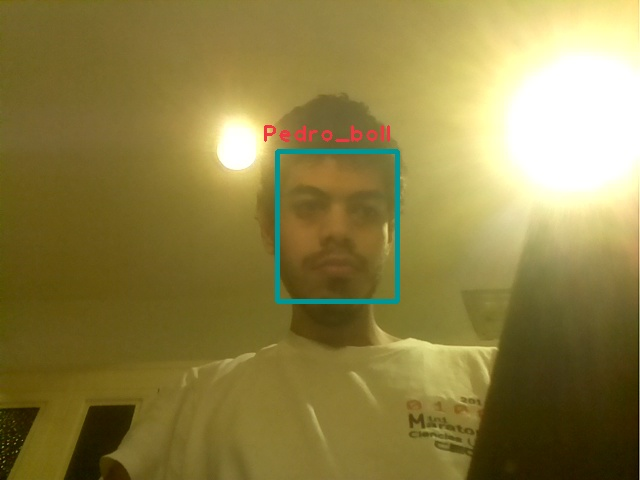
\includegraphics[scale=0.2]{./Figuras/IA_Pedro.jpeg}
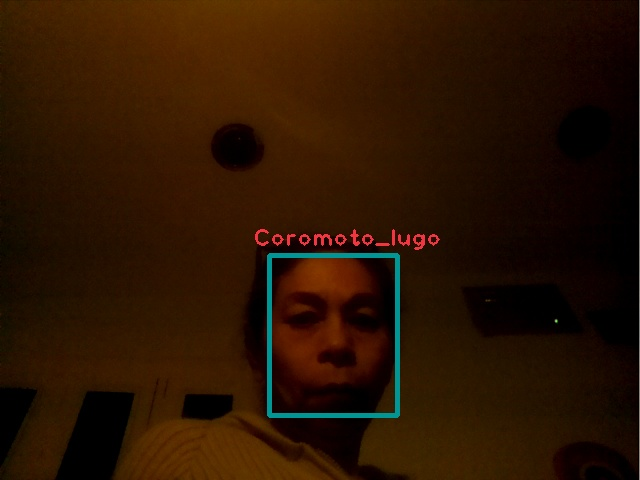
\includegraphics[scale=0.2]{./Figuras/IA_Coromoto.jpeg}
\caption{Identificación de rostros usando un modelo de IA desplegado en un Raspberry Pi 3 modelo B}
\label{fig:ia_rip3}
\vspace*{-10pt}
\end{figure}

\end{itemize}

\subsubsection{Variedad en los sensores}
Dada la redundancia de algunos sensores que medían el mismo tipo de variables ambientales y teniendo en cuenta el item anterior se quiso observar las diferencias en la representación, desempeño y facilidad de utilizar y mantener, se estableció un pequeño estudio comparativo, seleccionando las variables de temperatura y el registro de luminosidad de la habitación para entender como las diferencias entre sensores puede afectar la data generada.\\ 

Particularmente esto se llevó a cabo del siguiente modo: Haciendo uso de la placa programable Arduino Uno se decidió construir el prototipo de dispositivo IoT con el sensor de Temperatura DS1820 y la utilización de una fotorresistencia (LDR) para medir la intensidad de la luz. Por otro lado con una de las placas Raspberry Pi 3 Modelo B le fueron conectados un sensor de Temperatura (y humedad) DHT11, así como también un sensor de medición de intensidad TSL2561. Los resultados de la comparación fueron: 
\begin{itemize}
\item En cuanto a los sensores de temperatura se vieron que ambo sensores de temperatura tanto el DHT11 como el DS1820 (figura \ref{fig:sensores_temp}) fueron capaz de hacer lecturas del ambiente bajo el margen de error de los fabricantes. Sin embargo es importante recalcar que el sensor DS1820 fue mucho más preciso en la medición que el sensor DHT11. Esto se puede explicar por las especificaciones de cada tipo de sensor. Otra diferencia es en la manera y velocidad que se reflejaban los datos de los mismos, siendo más rápido el sensor DS1820 al momento de hacer lecturas que el sensor DHT11, siendo su dato un número de punto flotante versus un tipo de dato complejo que se genera en el sensor DHT11, siendo esto explicado que este último también lee en el mismo margen de tiempo la humedad ambiental. Ambos sensores representaban la temperatura en grados centigrados.

\begin{figure}[htb]
\centering
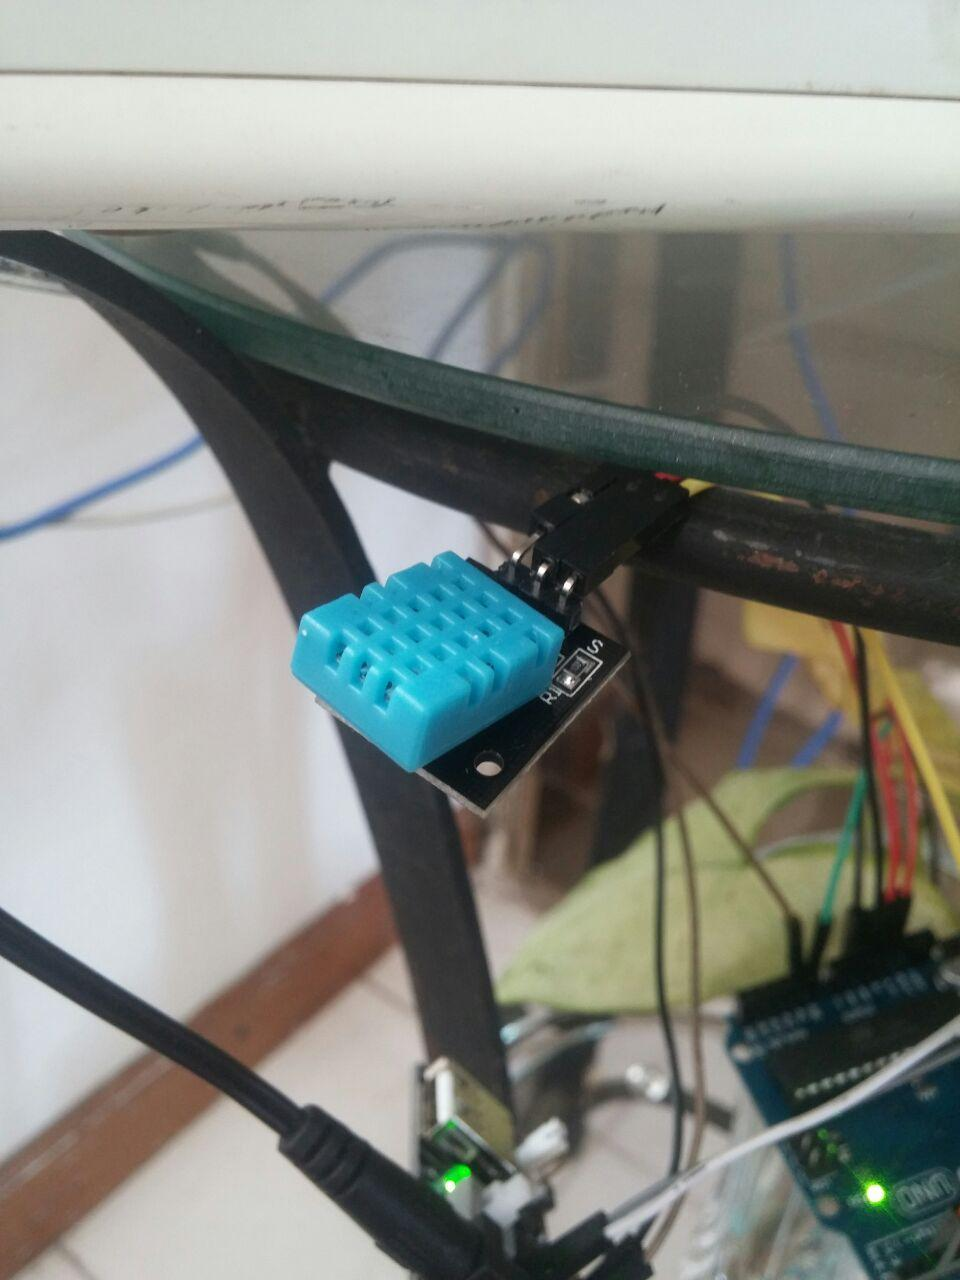
\includegraphics[scale=0.18]{./Figuras/temp_ext.jpg}
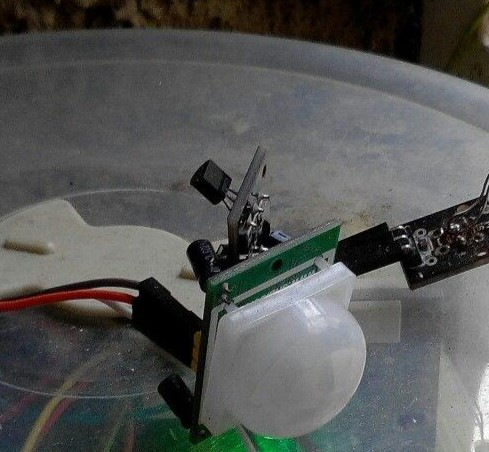
\includegraphics[scale=0.38]{./Figuras/ds1820.jpg}
\caption{A la izquierda el sensor de temperatura y humedad DHT11 y a la derecha el sensor de temperatura DS1820}
\label{fig:sensores_temp}
\vspace*{-10pt}
\end{figure}

\item Con respecto a la variable de intensidad lumínica en la habitación se compararon una fotorresistencia (LDR) simple contra un sensor TSL2561. A pesar de que ambos buscan el mismo objetivo, la fotorresistencia arroja valores que deben ser interpretados, pues inicialmente este representa la resistencia de una corriente eléctrica y teniendo ese valor se puede calcular la cantidad de luz disponible en el ambiente, mientras que el sensor TSL2561 directamente registra un valor en lux, que es una unidad directa de nivel de iluminación. Ambos valores del tipo numérico con la diferencia que el sensor TSL2561 usa valores de punto flotante y la fotorresistencia registra valores entre 0 y 1023 en el dispositivo Arduino.   
\end{itemize}

Otro punto importante dentro de la variedad de los sensores y actuadores es el formato de los distintos datos generados. Se pudo constatar que dependiendo de del tipo de sensor los formatos y los valores de los datos es bastante variado, lo suficiente como para concluir que es una potencial debilidad y que se deben utilizar métodos adecuados para poder tratar con ellos. Esto se vio reflejados en elecciones que se podrán observar en la siguiente parte de los escenarios de prueba. 

\subsection{Aplicación HAMACA}
En el caso de la aplicación web HAMACA las pruebas consistieron en poder obtener gestionar los datos e información generados de dispositivos, y dar opciones de control y monitoreo de los mismos así como también en ofrecer a los usuarios la flexibilidad y facilidad de uso sobre las herramientas integradas, todo esto haciendo uso de una navegación sencilla sobre las interfaces. 

\subsubsection{Captura de Información}
En términos de la captura de información y como parte del modulo de Redes desarrollado dentro de la aplicación se creo un script que es capaz de poder hacer las lecturas de tópicos para aquellos mensajes MQTT que llegacen al broker. Dichos mensajes generan dos elementos claves para la operación de esta solución:
\begin{itemize}
\item Guardar en la base de datos InfluxDB el dato que está siendo recibido para fines de visualización en tiempo real y almacenamiento histórico para su posterior análisis (figura \ref{fig:captura_data}).
\begin{figure}[htb]
\centering
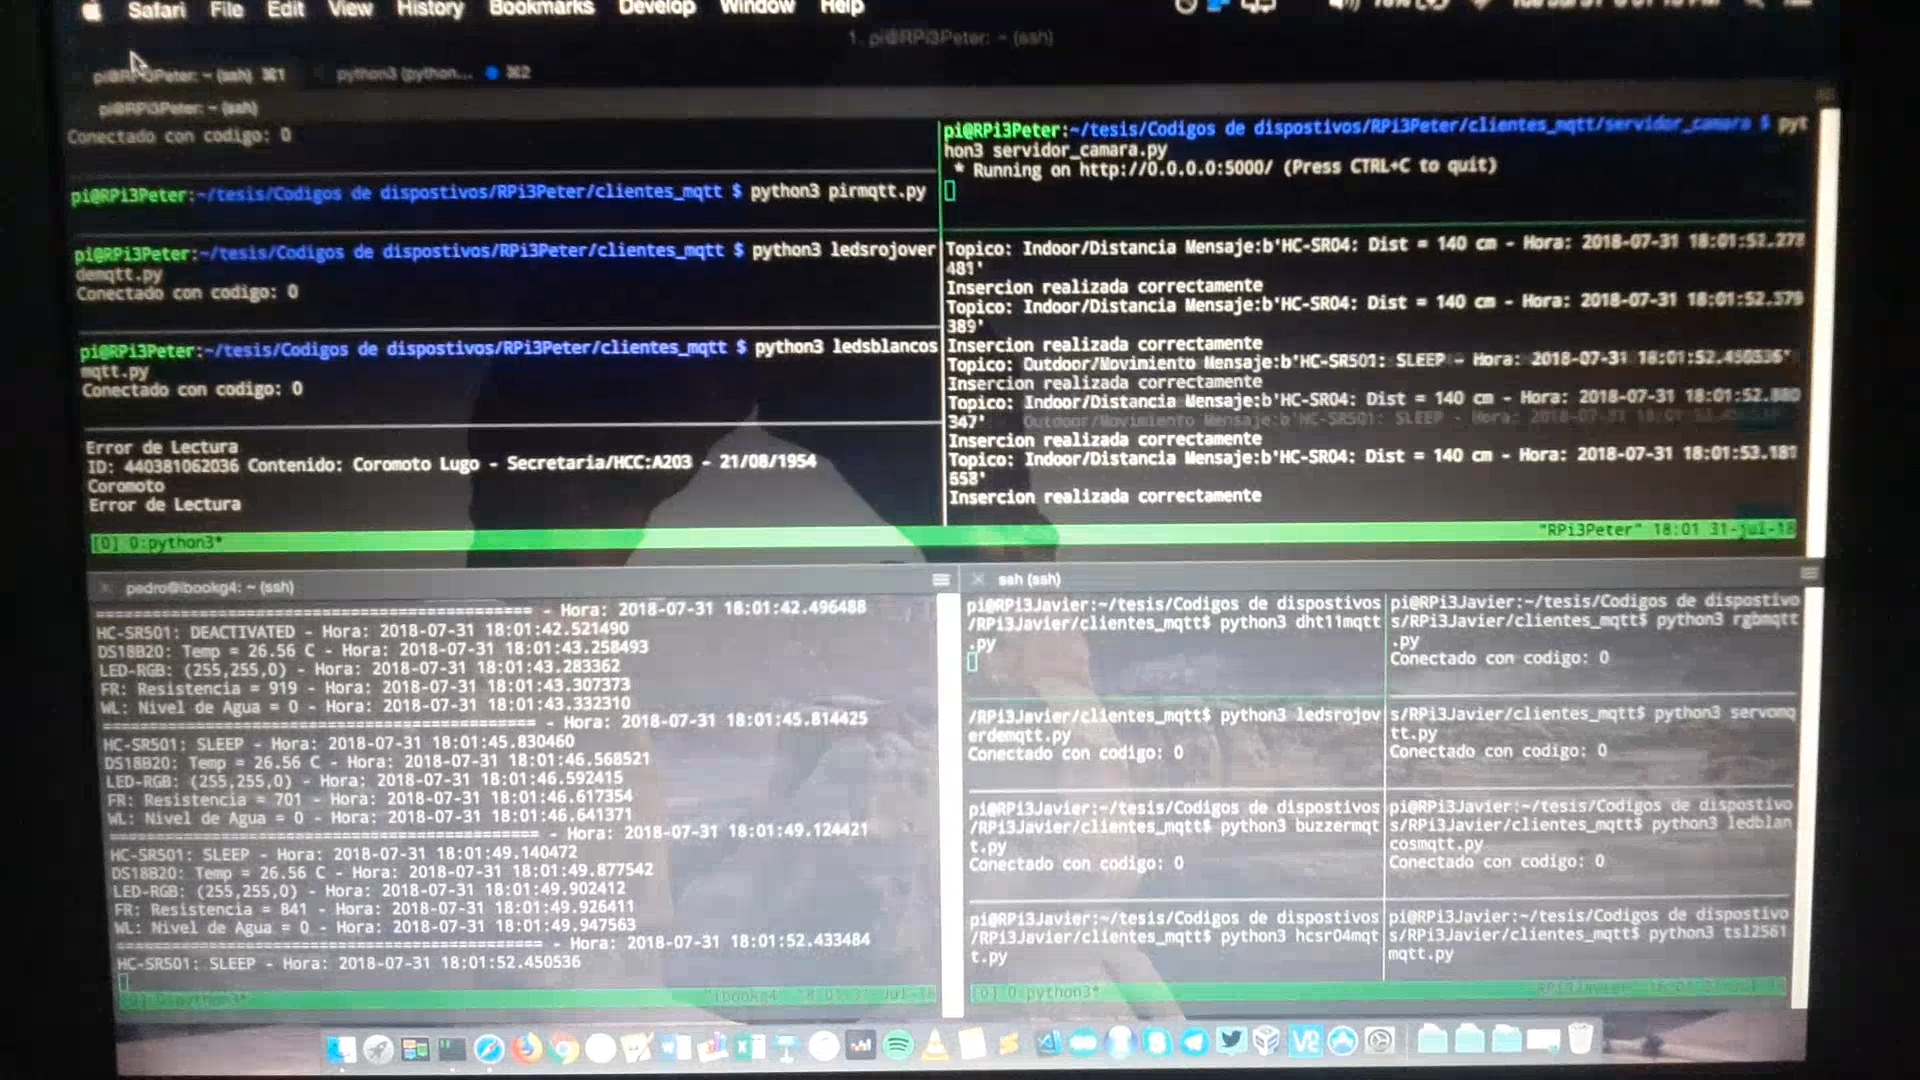
\includegraphics[scale=0.18]{./Figuras/captura_data.png}
\caption{Captura de datos por parte del backend de la aplicación web}
\label{fig:captura_data}
\end{figure}

\item Guardar estadísticas de uso, tópicos y contenido de mensajes recibidos por el broker como parte de la aplicación en la base de datos Postgresql (figura \ref{fig:app_red}).
\begin{figure}[htb]
\centering
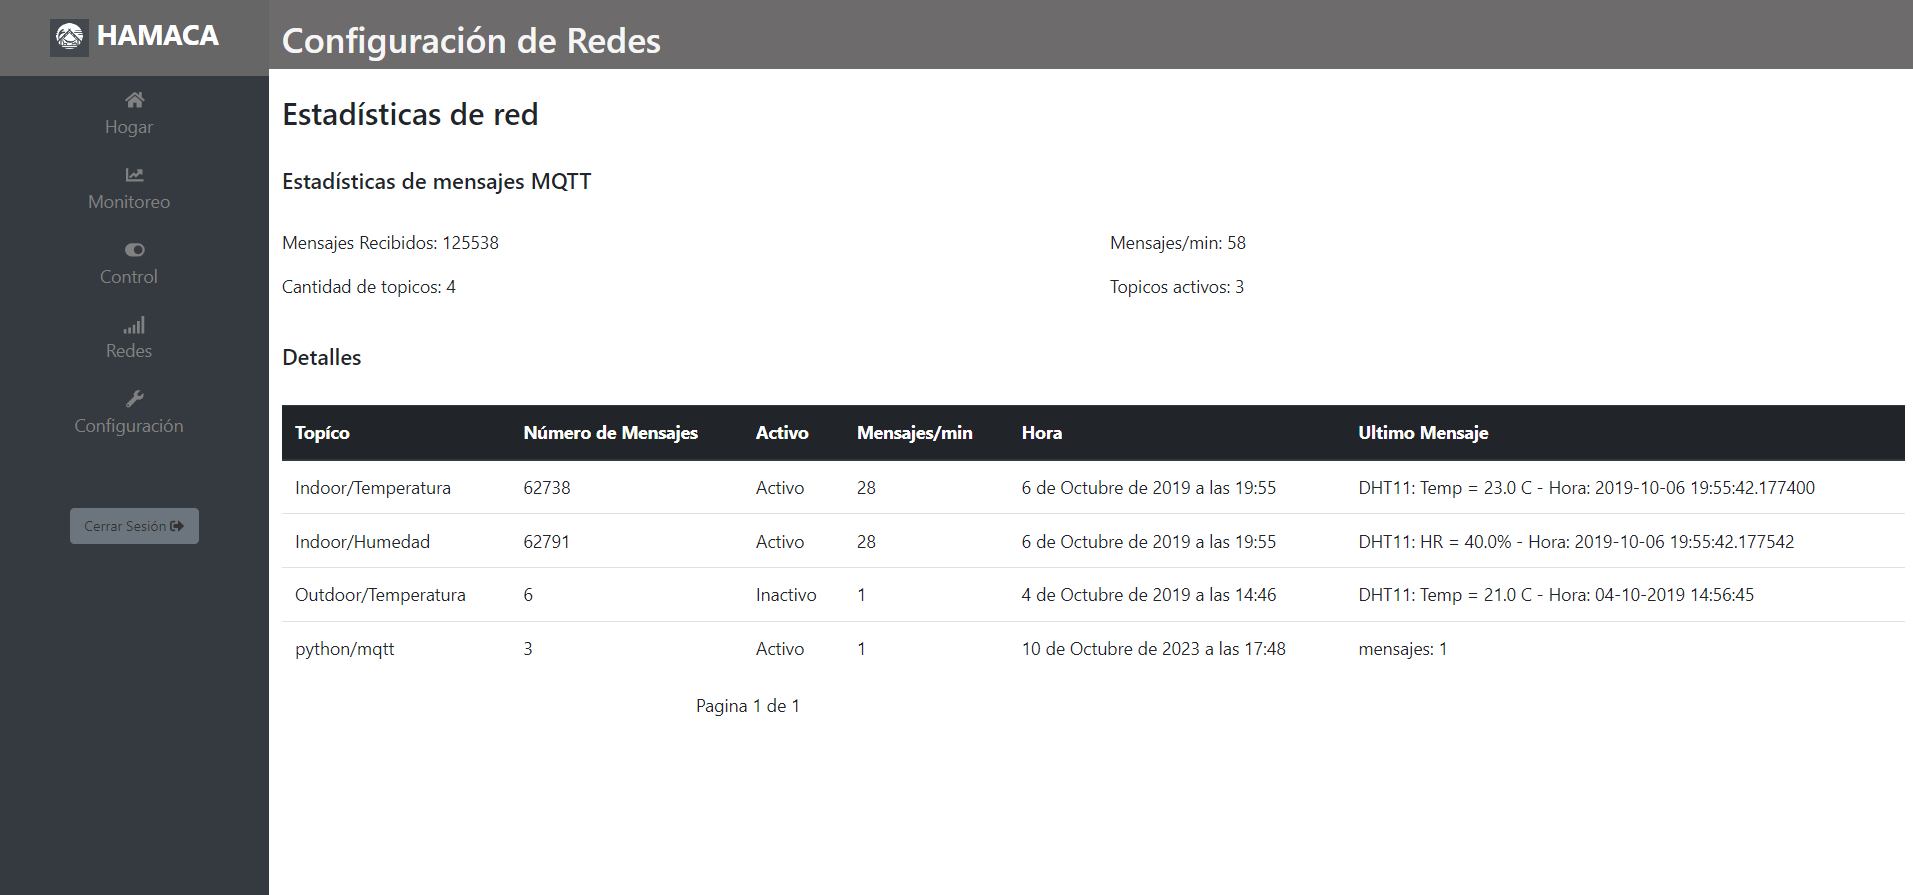
\includegraphics[scale=0.2]{./Figuras/hamaca_redes.png}
\caption{Estadísticas de mensajería del broker MQTT}
\label{fig:app_red}
\vspace*{-10pt}
\end{figure}
\end{itemize} 

Se pudo observar como en ambas instancias este script cuya función es hacer un proceso de extracción, transformación y carga (ETL), además de hacer la inserción en ambas bases de datos utilizadas, proceso crítico como parte de la ingesta de datos que luego se procesa en las herramientas integradas como en la propia aplicación. 

\subsubsection{Visualización de datos}
En la parte de visualización de datos, la evaluación de la aplicación web correspondía si a las funcionalidades de la herramienta de visualización de datos que se integro (Grafana) era lo suficientemente robusta y genérica para poder cumplir con los objetivos buscados.\\

La primera funcionalidad es la rápida y fácil integración con la fuente de datos, es decir, con el sistema manejador de base de datos InfluxDB. Este proceso es bastante sencillo y la herramienta también presenta una gran variedad distinta de otras fuentes de datos posibles. Una vez configurado ese aspecto, se puede ir directamente sobre la opción de crear un cuadro de mando o dashboard en el cual se puede agregar todo tipo de elementos que van desde multiples tipos de gráficos, textos, representaciones visuales e incluso, la posibilidad de embeber otros elementos de otras fuentes. Así es posible generar cuadros de mando altamente personalizados de manera muy sencilla.\\

Al momento de crear un gráfico, Grafana nos provee con una interfaz en donde realizar la consulta a la fuente de datos configurada (en este caso, la base de datos InfluxDB) haciendo uso de las consultas nativas de la fuente como se puede observar en la figura \ref{fig:consulta_grafana}.\\
\begin{figure}[htb]
\centering
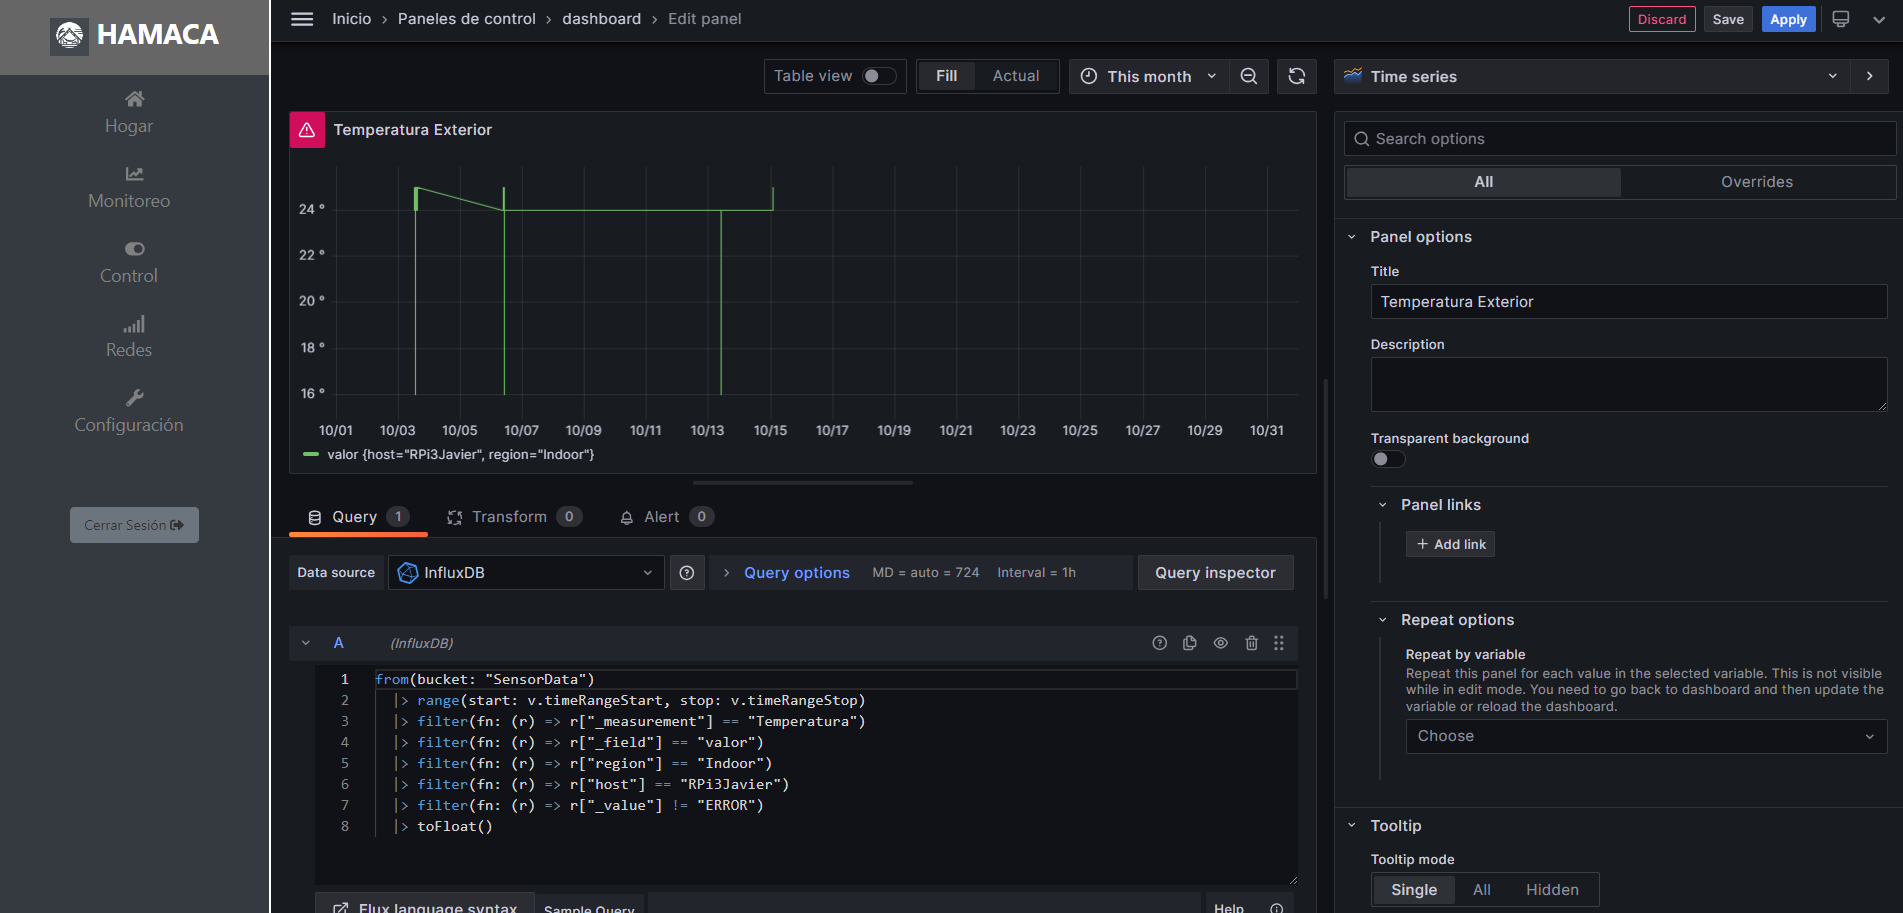
\includegraphics[scale=0.225]{./Figuras/consulta_grafana.png}
\caption{Consulta para construcción de gráficos usando la integración de Grafana}
\label{fig:consulta_grafana}
\vspace*{-10pt}
\end{figure}

Este es el principal problema que posee la herramienta pues hace que el usuario conozca el como consultar  los datos que quiera representar. Si no conoce la naturaleza de los mismos, la herramienta no tiene la posibilidad de ayudar a construir la información. Particularmente InfluxDB en su versión 2.0 cambio el lenguaje de consulta por uno llamado "flux" que lamentablemente es más complejo que su contraparte anterior lo cual puede elevar la curva de aprendizaje sobre la herramienta.\\

Sin embargo la potencia y flexibilidad ofrecida por Grafana la hace una herramienta idonea tanto para la vista de datos en tiempo real, como información histórica y junto con InfluxDB que al ser una base de datos basada en series de tiempo, definitivamente es una combinación que puede brindar información significativa y conocimiento accionable a través del análisis que se puede realizar sobre los diversos elementos que proveen los cuadros de mando como se puede ver en la figura \ref{fig:hamaca_grafana_panel}.  
\begin{figure}[htb]
\centering
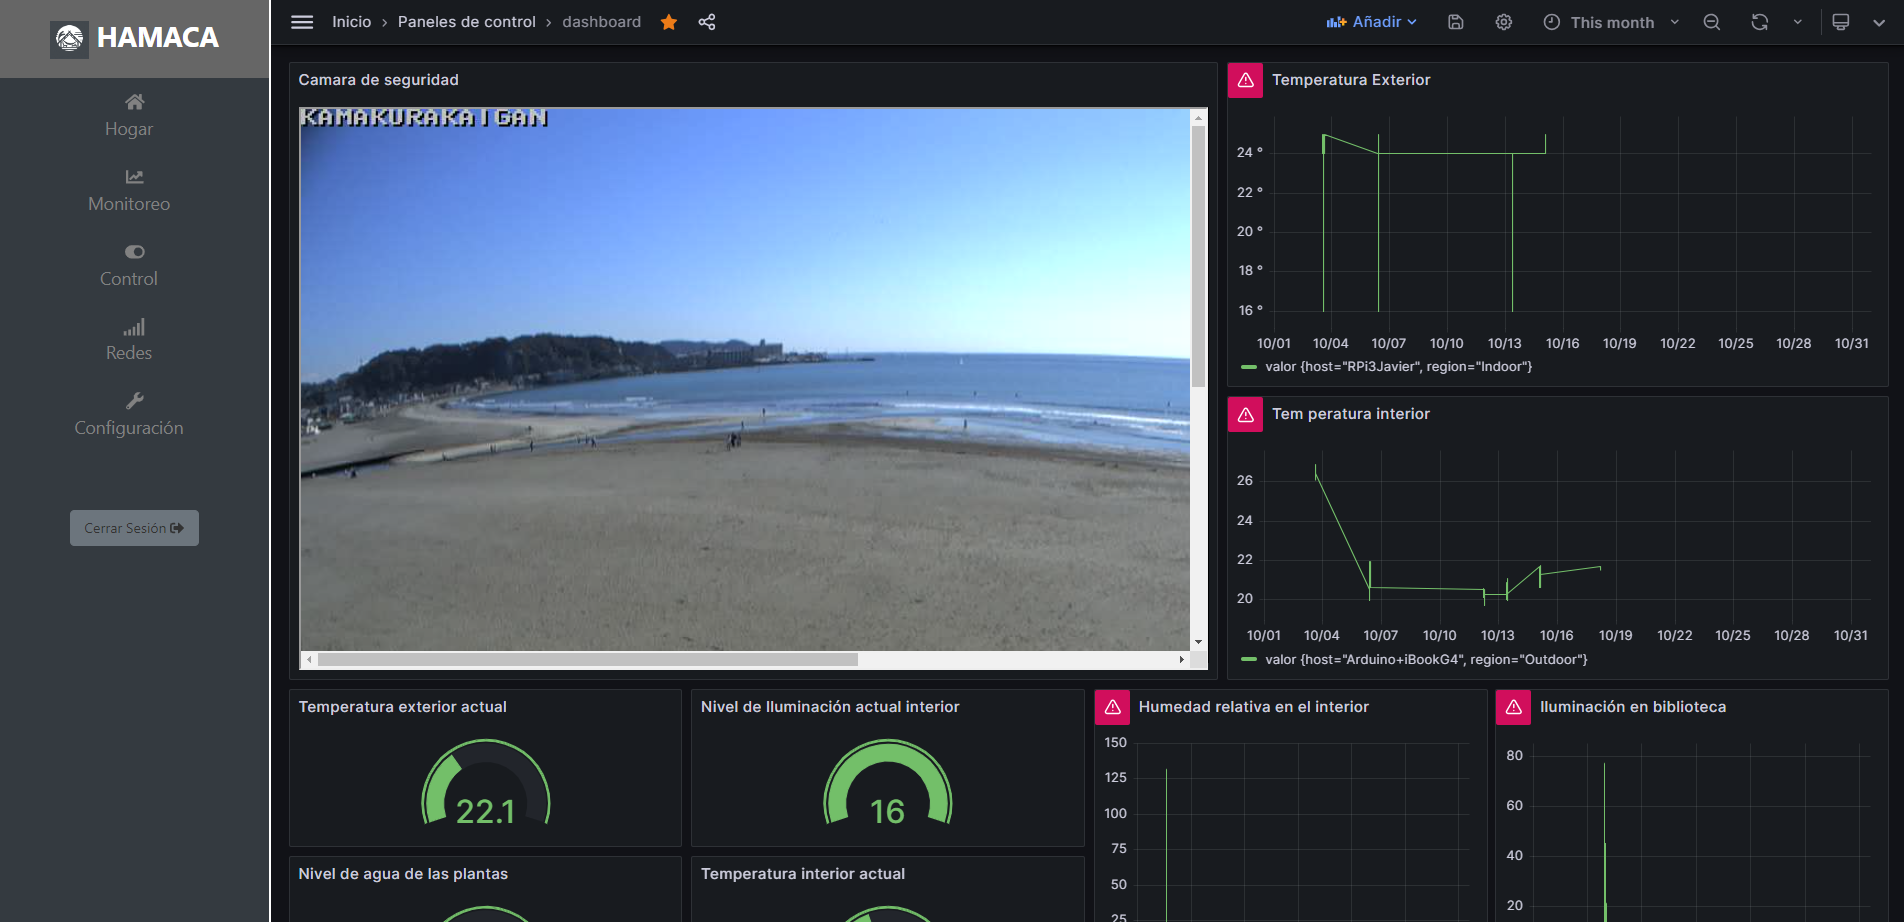
\includegraphics[scale=0.23]{./Figuras/hamaca_grafana_panel.png}
\caption{Cuadro de Mando con indicadores de la integración con Grafana}
\label{fig:hamaca_grafana_panel}
\vspace*{-10pt}
\end{figure}

\subsubsection{Monitoreo de Dispositivos}
Para el caso del monitoreo (y del control) la aplicación web ha hecho uso de la integración de la herramienta Node-Red, la cual fue diseñada para poder brindar flujos de automatización a dispositivos IoT más allá de su programación inicial. Con ellos se pueden crear ``flujos'' con los que poder extender comportamientos y automatizar una infinidad de aspectos sobre ellos. 

Cuando se crean uno ó más ``flujos", estos pueden llevar a un cuadro de mando con interfaces que permiten generar controles sobre los dispositivos siguiendo la receta anteriormente creada. Estos se despliegan como parte del Home de la aplicación web donde se resume de manera intuitiva para los usuarios (figura \ref{fig:node_red_ui}), teniendo la posibilidad de asignar flujos a diferentes cuadros de mando que se pueden acceder desde esa opción.\\

\begin{figure}[htb]
\centering
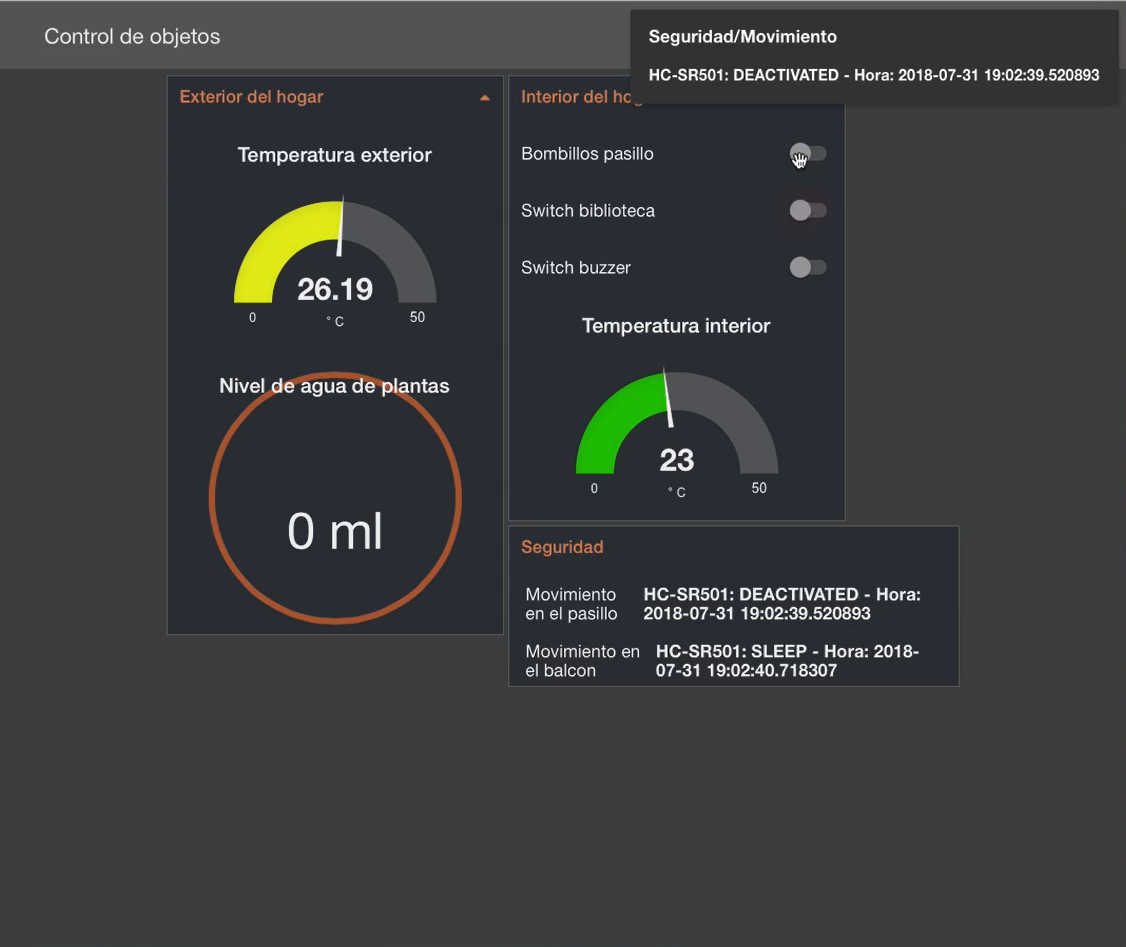
\includegraphics[scale=0.315]{./Figuras/node_red_ui.png}
\caption{Cuadro de Mando con indicadores e interfaces de control de dispositivos}
\label{fig:node_red_ui}
\vspace*{-10pt}
\end{figure}

Se pudo comprobar que creando el flujo desde la interfaz del cuadro de mando hacia el broker MQTT (como se explicará en el siguiente apartado) que efectivamente se podían controlar los elementos accionables de los actuadores de los prototipos, logrando así que los usuarios puedan también bajo demanda utilizar las funcionalidades de dispositivos IoT.

\subsubsection{Control de Dispositivos}
Finalmente para el control de los dispositivos se estableció que aplicación (a través de la integración de Node-Red) fuese capaz de poder crear formas de control (manual o automatizada) de los prototipos que fueron creados.\\

Para tal objetivo se crearon una serie de flujos que no solo sirvieran para poder establecer la interfaz de monitoreo sino también para poder automatizar una seríe de elementos representados por recursos de seguridad como lo fueron la presencia de movimiento en el exterior del hogar, el no reconocimiento de un rostro por parte del modelo de inteligencia artificial en la cámara del Raspberry Pi 3 modelo B, la notificación de una temperatura muy baja o muy alta para abrir o cerrar las ventanas o la notificación de la poca o nula presencia de agua por parte del sensor de nivel de agua en el exterior.\\

Como se puede notar en la figura \ref{fig:hamaca_nodered} estos elementos son creados a partir de pasos visuales, que luego requieren cierta configuración interna para poder funcionar correctamente. En la mayoría de los casos no se requiere de ningún conocimiento previo, pero por otro lado, elementos puntuales de transformación de datos y el manejo de comunicación requiere tanto conocimientos de programación(en el lenguaje javascript) como de como funcionan los protocolos o la infraestructura en la cual se soportan dichos servicios, lo cual puede desanimar a la mayoría de los usuarios de realizar tareas de automatización más complejas.
\begin{figure}[htb]
\centering
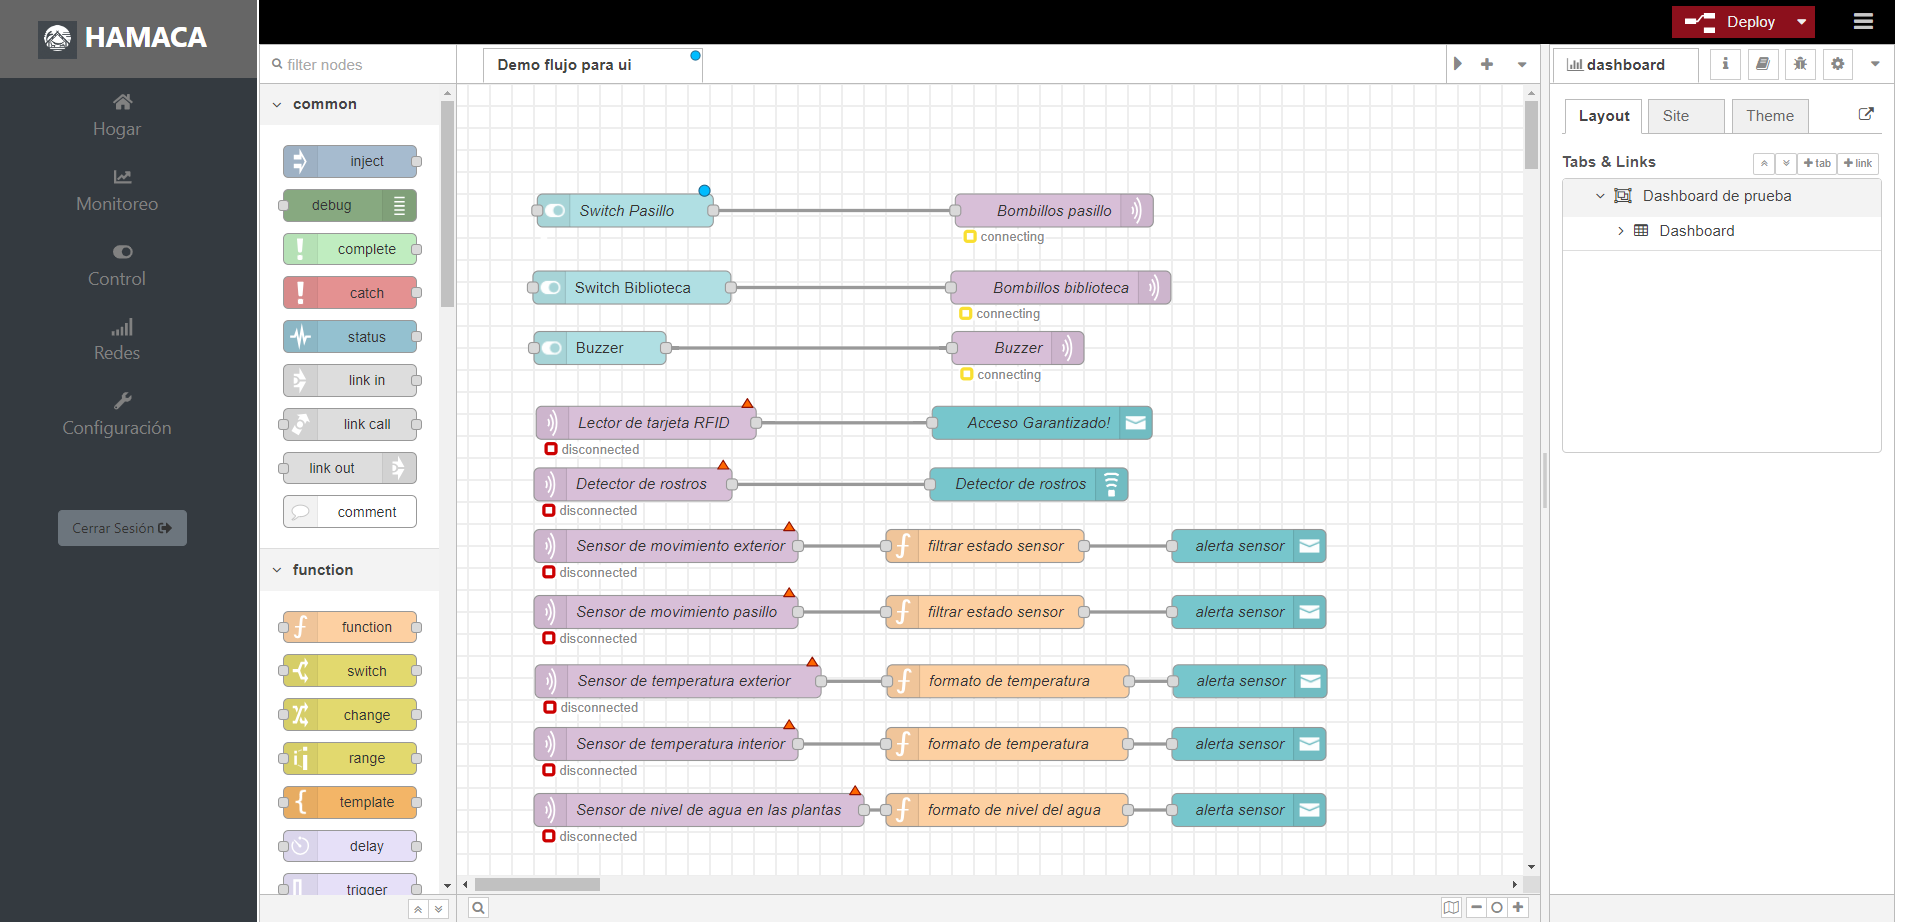
\includegraphics[scale=0.225]{./Figuras/hamaca_nodered.png}
\caption{Flujos creados dentro de la integración de Node-Red para automatizar tareas}
\label{fig:hamaca_nodered}
\vspace*{-10pt}
\end{figure}